% ============================================================
% CHAPTER 6 - RESULTS AND EVALUATION
% ============================================================
\chapter{Results and Evaluation}
\label{ch:results}

\section{Introduction}

This chapter reports and analyses the results. Section~\ref{sec:res-dataset}
covers dataset construction and the resulting label distribution.
Section~\ref{sec:res-training} reports training behaviour.
Section~\ref{sec:arch-comparison} presents the architecture comparison that
answers RQ3. Sections~\ref{sec:res-selected} and \ref{sec:res-imbalance} analyse
the selected model in detail, including the low precision observed under the
natural class distribution. Section~\ref{sec:per-phoneme} presents the
per-phoneme error profile (RQ4) and Section~\ref{sec:res-separation} the
control-versus-dysarthric separation that answers RQ2.
Sections~\ref{sec:qualitative} and \ref{sec:res-system} evaluate the deployed
system, and Sections~\ref{sec:discussion} and \ref{sec:limitations} discuss the
findings and state the limitations.

\section{Dataset Construction Results}
\label{sec:res-dataset}

Ten thousand dysarthric--control recording pairs were processed. Three pairs
failed, all at the alignment stage and all for the same reason: the target
phoneme sequence was longer than the number of CTC emission frames available,
which makes the constrained path set of Equation~\eqref{eq:ctc-align} empty. A
failure rate of $0.03\%$ indicates that the G2P and alignment stages are
essentially robust on this corpus. Table~\ref{tab:dataset-stats} summarises the
resulting corpus.

\begin{table}[H]
\centering
\caption[Dataset construction statistics]{Dataset construction statistics.}
\label{tab:dataset-stats}
\begin{tabular}{@{}lr@{}}
\toprule
\textbf{Quantity} & \textbf{Value} \\
\midrule
Recording pairs processed              & 10{,}000 \\
Pairs failed at alignment              & 3 \\
Control phoneme instances              & 49{,}153 \\
Dysarthric phoneme instances           & 49{,}153 \\
\textbf{Total labelled phoneme instances} & \textbf{98{,}306} \\
\midrule
Minimum deviation $D$                  & 0.13\,dB \\
Median deviation $D$                   & 0.76\,dB \\
Maximum deviation $D$                  & 6.83\,dB \\
Error cutoff $\tau$ (top 30\% of dysarthric) & 1.20\,dB \\
\midrule
Global mel mean $\mu$                  & $-2.41$\,dB \\
Global mel standard deviation $\sigma$ & 10.22\,dB \\
\bottomrule
\end{tabular}
\end{table}

The deviation distribution is strongly right-skewed: the median of $0.76$\,dB
sits well below the midpoint of the $[0.13, 6.83]$ range, so most dysarthric
phonemes deviate only mildly from their control counterparts while a long tail
deviates severely. This is consistent with the clinical picture that even
substantially impaired speakers produce many phonemes acceptably, and it is
precisely the structure that Method~1 destroyed by imposing a fixed quota over
the pooled distribution.

\subsection{Resulting label distribution}

\begin{table}[H]
\centering
\caption[Label distribution under Method 2]{Label distribution produced by the
control-baseline labelling rule.}
\label{tab:label-dist}
\begin{tabular}{@{}lrrr@{}}
\toprule
\textbf{Source} & \textbf{Correct (0)} & \textbf{Error (1)} & \textbf{Total} \\
\midrule
Control instances    & 49{,}153 & 0        & 49{,}153 \\
Dysarthric instances & 34{,}407 & 14{,}746 & 49{,}153 \\
\midrule
\textbf{Total}       & \textbf{83{,}560} & \textbf{14{,}746} & \textbf{98{,}306} \\
\textbf{Proportion}  & \textbf{85.0\%}   & \textbf{15.0\%}   & \\
\bottomrule
\end{tabular}
\end{table}

Table~\ref{tab:label-dist} exhibits the three properties predicted in
Section~\ref{sec:method2}. The control row contains \emph{no} errors, by
construction. Of the dysarthric instances, 70.0\% are labelled correct, which
means the model is never taught the spurious rule ``impaired speaker implies
error''. And the resulting class balance of 15.0\%/85.0\% is emergent from the
data rather than imposed: under Method~1 the error proportion would have been
exactly $30\%$ of the whole corpus by definition, including roughly
$30\%$ of all control instances.

\subsection{Data partitioning}

\begin{table}[H]
\centering
\caption[Data partitioning]{Data partitioning. Balancing is applied to the
training partition only.}
\label{tab:split}
\small
\begin{tabular}{@{}lrrp{5.4cm}@{}}
\toprule
\textbf{Partition} & \textbf{Instances} & \textbf{Error \%} & \textbf{Treatment} \\
\midrule
Training (raw)      & 78{,}644  & 15.0\% & 80\% stratified split \\
Training (balanced) & 133{,}694 & 50.0\% & Minority upsampled with replacement \\
Held-out test       & 19{,}662  & 15.0\% & Natural distribution, untouched \\
\bottomrule
\end{tabular}
\end{table}

The held-out partition contains 2{,}949 error and 16{,}713 correct instances.
Retaining the natural distribution is deliberate: it is the distribution the
deployed model will encounter, and evaluating on an artificially balanced test
set would report a precision that the system cannot achieve in service.

\section{Training Behaviour}
\label{sec:res-training}

Training ran for 12 epochs before early stopping, with the best validation loss
of $0.4786$ reached at epoch 7 and those weights restored.
Figure~\ref{fig:training-curves} shows the accuracy and loss trajectories.

\begin{figure}[H]
\centering
\begin{tikzpicture}
\begin{groupplot}[
  group style={group size=2 by 1, horizontal sep=18mm},
  width=0.48\textwidth, height=6.0cm,
  xlabel={Epoch}, xmin=1, xmax=12, xtick={1,2,...,12},
  grid=major, grid style={gray!22},
  tick label style={font=\scriptsize}, label style={font=\scriptsize},
  title style={font=\small}, legend style={font=\tiny, draw=none, fill=white,
  fill opacity=0.85, text opacity=1},
]

\nextgroupplot[ylabel={Accuracy}, ymin=0.58, ymax=0.76, title={Accuracy},
               legend pos=south east]
\addplot[thick, blue!70!black, mark=*, mark size=1.2pt] coordinates {
  (1,0.6495)(2,0.6842)(3,0.6987)(4,0.7079)(5,0.7136)(6,0.7174)
  (7,0.7203)(8,0.7251)(9,0.7289)(10,0.7315)(11,0.7346)(12,0.7364)};
\addlegendentry{train}
\addplot[thick, red!70!black, mark=square*, mark size=1.2pt] coordinates {
  (1,0.6164)(2,0.6045)(3,0.6336)(4,0.6376)(5,0.6638)(6,0.6891)
  (7,0.7199)(8,0.6198)(9,0.6809)(10,0.6546)(11,0.6629)(12,0.6814)};
\addlegendentry{validation}
\draw[dashed, black!70] (axis cs:7,0.58) -- (axis cs:7,0.76);
\node[font=\tiny, anchor=south west, rotate=90] at (axis cs:7.05,0.585) {best epoch};

\nextgroupplot[ylabel={Loss}, ymin=0.45, ymax=0.65, title={Loss},
               legend pos=north east]
\addplot[thick, blue!70!black, mark=*, mark size=1.2pt] coordinates {
  (1,0.6257)(2,0.5899)(3,0.5725)(4,0.5601)(5,0.5545)(6,0.5456)
  (7,0.5396)(8,0.5341)(9,0.5273)(10,0.5234)(11,0.5185)(12,0.5149)};
\addlegendentry{train}
\addplot[thick, red!70!black, mark=square*, mark size=1.2pt] coordinates {
  (1,0.6158)(2,0.6031)(3,0.5721)(4,0.5812)(5,0.5592)(6,0.5029)
  (7,0.4786)(8,0.5556)(9,0.5165)(10,0.5179)(11,0.5175)(12,0.5055)};
\addlegendentry{validation}
\draw[dashed, black!70] (axis cs:7,0.45) -- (axis cs:7,0.65);
\node[font=\tiny, anchor=south west, rotate=90] at (axis cs:7.05,0.455) {best epoch};
\end{groupplot}
\end{tikzpicture}
\caption[Training and validation curves]{Training and validation accuracy and
loss over 12 epochs. Early stopping restored the epoch-7 weights, at which the
validation loss was minimal (0.4786).}
\label{fig:training-curves}
\end{figure}

Three features of Figure~\ref{fig:training-curves} deserve comment.

\textbf{Training accuracy rises smoothly and modestly}, from 64.95\% to 73.64\%
over 12 epochs, with no sign of the sharp climb towards the high nineties that
would indicate memorisation. Given a 415{,}810-parameter model and 133{,}694
training instances, this is the expected profile for a task whose labels carry
genuine noise: the model is fitting the signal that exists and is prevented by
dropout from fitting the rest.

\textbf{Validation accuracy is markedly non-monotonic}, oscillating between
60.45\% and 71.99\%. Two causes are identifiable. The training set is balanced
50/50 while the validation set is at the natural 15/85, so a small shift in the
decision boundary produces a large change in validation accuracy through the
majority class. Additionally, the labels themselves are proxy labels derived
from a distance threshold, and instances near that threshold are intrinsically
ambiguous; their predictions flip readily between epochs.

\textbf{The train--validation loss gap remains small}, and validation loss is
below training loss for much of the run. This is a consequence of dropout being
active during training and inactive during evaluation, and it confirms that the
model is not overfitting. The best validation loss at epoch 7 coincides with the
best validation accuracy, so early stopping selected a well-behaved point rather
than an artefact.

\section{Architecture Comparison}
\label{sec:arch-comparison}

Five architectures were trained and evaluated under the common protocol of
Table~\ref{tab:hyperparams}, differing only in the temporal-modelling stage.
Results are given in Table~\ref{tab:arch-comparison} and
Figure~\ref{fig:arch-comparison}.

\begin{table}[H]
\centering
\caption[Architecture comparison]{Comparison of candidate architectures. All
metrics for the error class except accuracy. Best value in each column is
shown in bold.}
\label{tab:arch-comparison}
\begin{tabular}{@{}lrrrr@{}}
\toprule
\textbf{Model} & \textbf{Accuracy} & \textbf{Precision} & \textbf{Recall} & \textbf{$F_1$} \\
\midrule
CNN--BiLSTM & 73.13\% & 71.61\% & \textbf{76.64\%} & \textbf{74.04\%} \\
CNN--LSTM   & 73.13\% & 72.03\% & 75.62\%          & 73.78\% \\
CNN--BiGRU  & \textbf{73.40\%} & \textbf{74.19\%} & 71.75\% & 72.95\% \\
CNN         & 70.50\% & 71.40\% & 68.40\%          & 69.86\% \\
CNN--GRU    & 69.65\% & 73.53\% & 61.41\%          & 66.93\% \\
\bottomrule
\end{tabular}
\end{table}

\begin{figure}[H]
\centering
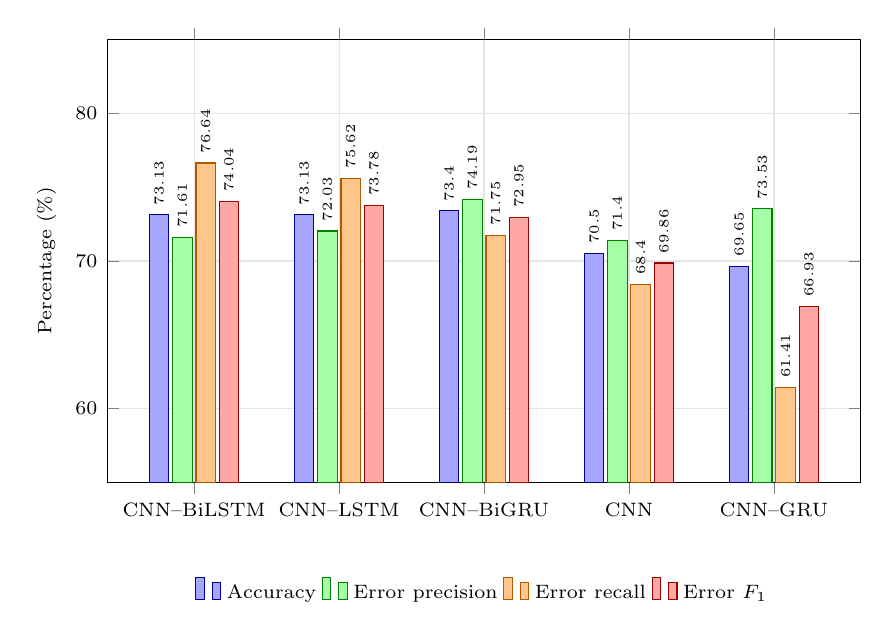
\begin{tikzpicture}
\begin{axis}[
  width=0.92\textwidth, height=7.2cm,
  ybar=1.4pt, bar width=7pt,
  ymin=55, ymax=85,
  ylabel={Percentage (\%)},
  xmin=0.4, xmax=5.6,
  xtick={1,2,3,4,5},
  xticklabels={CNN--BiLSTM, CNN--LSTM, CNN--BiGRU, CNN, CNN--GRU},
  tick label style={font=\scriptsize}, label style={font=\scriptsize},
  legend style={font=\scriptsize, at={(0.5,-0.20)}, anchor=north, legend columns=4, draw=none},
  grid=major, grid style={gray!20},
  nodes near coords, every node near coord/.append style={font=\tiny, rotate=90, anchor=west},
]
\addplot[fill=blue!35, draw=blue!60!black] coordinates {
  (1,73.13)(2,73.13)(3,73.40)(4,70.50)(5,69.65)};
\addlegendentry{Accuracy}
\addplot[fill=green!35, draw=green!50!black] coordinates {
  (1,71.61)(2,72.03)(3,74.19)(4,71.40)(5,73.53)};
\addlegendentry{Error precision}
\addplot[fill=orange!45, draw=orange!70!black] coordinates {
  (1,76.64)(2,75.62)(3,71.75)(4,68.40)(5,61.41)};
\addlegendentry{Error recall}
\addplot[fill=red!35, draw=red!60!black] coordinates {
  (1,74.04)(2,73.78)(3,72.95)(4,69.86)(5,66.93)};
\addlegendentry{Error $F_1$}
\end{axis}
\end{tikzpicture}
\caption[Architecture comparison chart]{Comparative performance of the five
candidate architectures.}
\label{fig:arch-comparison}
\end{figure}

\subsection{Interpretation}

\textbf{The recurrent stage contributes measurably.} The plain CNN, which omits
temporal modelling entirely, is the weakest model on both recall (68.40\%) and
$F_1$ (69.86\%), trailing the best recurrent model by 8.2 and 4.2 percentage
points respectively. This is the ablation that justifies the hybrid design: the
information the recurrent stage adds is the evolution of the spectro-temporal
features across the patch, which is where the quality of an articulatory gesture
resides.

\textbf{Bidirectionality helps the LSTM and hurts the GRU.} CNN--BiLSTM improves
on CNN--LSTM in recall ($+1.02$ points) and $F_1$ ($+0.26$ points) at identical
accuracy, whereas CNN--BiGRU differs from CNN--GRU far more dramatically:
bidirectionality lifts GRU recall from 61.41\% to 71.75\%, a gain of more than
ten points. The unidirectional GRU is the clear outlier of the study, with the
highest precision-to-recall imbalance of any candidate --- it is conservative,
predicting the error class rarely and being right when it does. Its low recall
makes it unsuitable for screening despite a respectable precision of 73.53\%.

\textbf{Accuracy does not discriminate.} The top three models span 0.27
percentage points of accuracy, which is well inside the run-to-run variation
expected from a single training run with a fixed seed. Accuracy alone would not
support a selection among them, which is the empirical justification for the
recall-based criterion adopted in Section~\ref{sec:arch-design}.

\subsection{Selection}

\textbf{CNN--BiLSTM was selected.} It attains the highest error-class recall
(76.64\%) and the highest error-class $F_1$ (74.04\%), which is exactly the
criterion stated in advance in Section~\ref{sec:arch-design}. The nearest
competitor on accuracy, CNN--BiGRU, trades 4.89 points of recall for 2.58 points
of precision and 0.27 points of accuracy --- an unfavourable exchange for a
screening tool, in which a missed error withholds the feedback the system exists
to provide while a false alarm costs one unnecessary repetition. CNN--LSTM is
very close behind CNN--BiLSTM and would be a reasonable alternative if
inference cost mattered more; it does not, at this model size.

\subsection{Note on evaluation protocol}

The figures in Table~\ref{tab:arch-comparison} come from the comparative study,
in which all five candidates were evaluated under a \emph{class-balanced}
evaluation set so that the four metrics are directly comparable across models
and are not dominated by the majority class. The detailed figures reported in
Section~\ref{sec:res-selected} for the deployed model are computed on the
\emph{naturally distributed} held-out partition of Table~\ref{tab:split}
(15\% error / 85\% correct). Accuracy and recall are broadly comparable between
the two protocols, but precision is not: precision depends directly on the class
prior, and the same classifier necessarily reports lower precision on a set in
which the positive class is rarer. The two tables should therefore be read as
answering different questions --- Table~\ref{tab:arch-comparison} answers
``which architecture separates the classes best'', and
Table~\ref{tab:classification-report} answers ``what will this model do in
service'' --- and their precision columns should not be compared directly.

\section{Performance of the Selected Model}
\label{sec:res-selected}

On the naturally distributed held-out partition the selected CNN--BiLSTM model
achieved an accuracy of \textbf{71.99\%}. The full classification report is
given in Table~\ref{tab:classification-report}.

\begin{table}[H]
\centering
\caption[Classification report on the held-out partition]{Classification report
for the selected model on the held-out partition (natural 15\%/85\%
distribution, 19{,}662 instances).}
\label{tab:classification-report}
\begin{tabular}{@{}lrrrr@{}}
\toprule
\textbf{Class} & \textbf{Precision} & \textbf{Recall} & \textbf{$F_1$} & \textbf{Support} \\
\midrule
Correct        & 0.94 & 0.71 & 0.81 & 16{,}713 \\
Error          & 0.32 & 0.75 & 0.45 & 2{,}949 \\
\midrule
Accuracy       &      &      & 0.72 & 19{,}662 \\
Macro average  & 0.63 & 0.73 & 0.63 & 19{,}662 \\
Weighted average & 0.85 & 0.72 & 0.76 & 19{,}662 \\
\bottomrule
\end{tabular}
\end{table}

The corresponding confusion matrix is shown in
Figure~\ref{fig:confusion-matrix}; its cell values are those consistent with the
reported accuracy, per-class recalls and supports.

\begin{figure}[H]
\centering
\begin{tikzpicture}[font=\small]
  \def\cw{3.1cm} \def\ch{1.7cm}
  \node[minimum width=\cw, minimum height=\ch, fill=blue!45, draw=black!60] (tn) at (0,0)
       {\color{white}\textbf{TN = 11{,}942}};
  \node[minimum width=\cw, minimum height=\ch, fill=blue!18, draw=black!60] (fp) at (3.3,0)
       {\textbf{FP = 4{,}771}};
  \node[minimum width=\cw, minimum height=\ch, fill=blue!6,  draw=black!60] (fn) at (0,-1.8)
       {\textbf{FN = 737}};
  \node[minimum width=\cw, minimum height=\ch, fill=blue!12, draw=black!60] (tp) at (3.3,-1.8)
       {\textbf{TP = 2{,}212}};

  \node[above=1mm of tn, font=\small\bfseries] {Predicted: Correct};
  \node[above=1mm of fp, font=\small\bfseries] {Predicted: Error};
  \node[left=2mm of tn, font=\small\bfseries, align=right, rotate=90] {True: Correct};
  \node[left=2mm of fn, font=\small\bfseries, align=right, rotate=90] {True: Error};

  \node[anchor=west, font=\scriptsize, align=left] at (5.3,-0.9)
       {Correct recall $= 11{,}942/16{,}713 = 0.71$\\
        Error recall $= 2{,}212/2{,}949 = 0.75$\\
        Error precision $= 2{,}212/6{,}983 = 0.32$\\
        Accuracy $= 14{,}154/19{,}662 = 0.72$};
\end{tikzpicture}
\caption[Confusion matrix]{Confusion matrix for the selected model on the
held-out partition. The error class is the positive class.}
\label{fig:confusion-matrix}
\end{figure}

\section{Analysis of Precision Under Class Imbalance}
\label{sec:res-imbalance}

The error-class precision of $0.32$ is the weakest number in this study and
requires an honest account. It means that roughly two of every three phonemes
the deployed model flags are, according to the derived labels, not errors.

\subsection{The class prior accounts for most of it}

Precision is a function of the base rate. The model produces 4{,}771 false
positives out of 16{,}713 true-correct instances --- a false-positive rate of
28.5\%. On a balanced evaluation set with 2{,}949 instances of each class, that
same false-positive rate would yield $2{,}949 \times 0.285 \approx 841$ false
positives against 2{,}212 true positives, for a precision of approximately
$0.72$ --- which is consistent with the 71.61\% reported for CNN--BiLSTM in
Table~\ref{tab:arch-comparison}. The classifier's discriminative behaviour is
therefore unchanged between the two protocols; what changes is the prior. When
85\% of instances are negative, even a moderate false-positive rate produces
more false positives than there are true positives available.

\subsection{Label noise accounts for part of it}

The remainder is attributable to the labels themselves. The ground truth is
derived from a threshold at $\tau = 1.20$\,dB on a continuous deviation
measure. A phoneme at $D = 1.19$\,dB is labelled correct and one at
$D = 1.21$\,dB is labelled an error, although they are acoustically
indistinguishable. Some proportion of the 4{,}771 ``false positives'' are
therefore instances that deviate substantially but fall just below the cutoff.
Because there is no clinician annotation available, this proportion cannot be
measured, and no claim is made about it beyond the observation that the true
precision against clinical ground truth is bounded below by the measured value
rather than equal to it.

\subsection{Why this operating point was nevertheless accepted}

Three considerations justify accepting the trade-off.

First, the criterion was fixed in advance (Section~\ref{sec:arch-design}) and
the asymmetry of costs is real: a false negative silently withholds feedback,
whereas a false positive costs one unnecessary repetition of a sound the user
was already practising.

Second, the operating point is user-adjustable. The threshold slider moves the
decision boundary within $[0.30, 0.70]$, so a user or clinician who prefers
precision to sensitivity can obtain it without retraining.

Third --- and most importantly --- the system-level quantity that matters is not
per-phoneme precision on a distance-derived label but whether the tool separates
clear from impaired speech at the level of a whole recording. That is the
subject of Section~\ref{sec:res-separation}, and it is the property that
distinguishes Method~2 from Method~1.

\section{Per-Phoneme Error Profile}
\label{sec:per-phoneme}

The model was applied to the full corpus and the predicted error rate computed
per IPA symbol, restricted to symbols occurring at least 100 times. Three rare
symbols fell below that count and were excluded as statistically unreliable. The
fifteen highest-rate symbols are given in Table~\ref{tab:per-phoneme} and
plotted in Figure~\ref{fig:per-phoneme}.

\begin{table}[H]
\centering
\caption[Per-phoneme predicted error rates]{Phonemes with the highest predicted
error rate (symbols with at least 100 occurrences).}
\label{tab:per-phoneme}
\begin{tabular}{@{}clrrl@{}}
\toprule
\textbf{Rank} & \textbf{Phoneme} & \textbf{Count} & \textbf{Error rate} & \textbf{Articulatory class} \\
\midrule
1  & \ph{ɾ} & 598   & 50.84\% & Alveolar flap \\
2  & \ph{ɚ} & 2{,}062 & 49.71\% & R-coloured (rhotic) vowel \\
3  & \ph{ŋ} & 674   & 46.44\% & Velar nasal \\
4  & \ph{ə} & 3{,}594 & 45.58\% & Reduced central vowel \\
5  & \ph{ʊ} & 4{,}122 & 44.30\% & Near-close back vowel \\
6  & \ph{z} & 1{,}744 & 44.09\% & Voiced alveolar fricative \\
7  & \ph{θ} & 706   & 43.77\% & Voiceless dental fricative \\
8  & \ph{v} & 1{,}270 & 43.46\% & Voiced labiodental fricative \\
9  & \ph{t} & 5{,}286 & 42.11\% & Voiceless alveolar stop \\
10 & \ph{l} & 4{,}562 & 41.34\% & Alveolar lateral approximant \\
11 & \ph{n} & 4{,}802 & 40.88\% & Alveolar nasal \\
12 & \ph{ɪ} & 8{,}534 & 40.05\% & Near-close front vowel \\
13 & \ph{ʒ} & 1{,}124 & 39.59\% & Voiced postalveolar fricative \\
14 & \ph{ɹ} & 4{,}352 & 39.11\% & Alveolar approximant \\
15 & \ph{m} & 2{,}646 & 38.28\% & Bilabial nasal \\
\bottomrule
\end{tabular}
\end{table}

\begin{figure}[H]
\centering
\begin{tikzpicture}
\begin{axis}[
  width=0.95\textwidth, height=6.6cm,
  ybar, bar width=11pt,
  ymin=0, ymax=55,
  ylabel={Predicted error rate (\%)},
  xlabel={Phoneme (IPA)},
  xmin=0.4, xmax=15.6,
  xtick={1,2,3,4,5,6,7,8,9,10,11,12,13,14,15},
  xticklabels={%
    {\textfishhookr},{\textrhookschwa},{\ng},{\textschwa},{\textupsilon},
    {z},{\texttheta},{v},{t},{l},{n},{\textsci},{\textyogh},{\textturnr},{m}},
  tick label style={font=\scriptsize}, label style={font=\scriptsize},
  grid=major, grid style={gray!20},
  nodes near coords, every node near coord/.append style={font=\tiny, rotate=90, anchor=west},
]
\addplot[fill=red!30, draw=red!60!black] coordinates {
  (1,50.84) (2,49.71) (3,46.44) (4,45.58) (5,44.30) (6,44.09) (7,43.77)
  (8,43.46) (9,42.11) (10,41.34) (11,40.88) (12,40.05) (13,39.59)
  (14,39.11) (15,38.28)};
\end{axis}
\end{tikzpicture}
\caption[Per-phoneme predicted error rates]{Predicted error rate by phoneme for
the fifteen most error-prone symbols with at least 100 occurrences.}
\label{fig:per-phoneme}
\end{figure}

\subsection{Clinical plausibility of the profile}

The ranking was not designed and is not an output the model was optimised for;
it is therefore usable as an external check on what the model has learned. Four
patterns in Table~\ref{tab:per-phoneme} align with the dysarthria literature
reviewed in Section~\ref{sec:lit-dysarthria}.

\textbf{Rapid, ballistic gestures rank highest.} The alveolar flap \ph{ɾ} is the
single most error-prone symbol at 50.84\%. A flap is a very brief ballistic
contact of the tongue tip, typically under 30\,ms, and it is exactly the class
of movement that impaired motor control cannot execute reliably. Its position at
the top of the ranking is the most articulatorily specific prediction the model
makes.

\textbf{Rhotics and reduced vowels rank high.} The rhotic schwa \ph{ɚ} (49.71\%),
schwa \ph{ə} (45.58\%) and the near-close vowels \ph{ʊ} (44.30\%) and \ph{ɪ}
(40.05\%) all appear in the top twelve, and the approximant \ph{ɹ} appears at
39.11\%. Rhotics require a precise and unusual tongue configuration and are
late-acquired even in typical development; reduced and near-close vowels sit
near the centre of the vowel space, and vowel-space compression
\cite{kim2011vowel} moves impaired productions towards precisely that region,
which makes them acoustically unstable.

\textbf{Fricatives are over-represented.} \ph{z} (44.09\%), \ph{θ} (43.77\%),
\ph{v} (43.46\%) and \ph{ʒ} (39.59\%) all appear despite being individually
less frequent than the stops and nasals. Fricatives require sustained precise
constriction to generate turbulent noise, and reduced airflow control degrades
them severely \cite{ansel1992acoustic}.

\textbf{Nasals appear where velopharyngeal control is implicated.} \ph{ŋ}
(46.44\%), \ph{n} (40.88\%) and \ph{m} (38.28\%) all rank in the top fifteen.
Hypernasality arising from incomplete velopharyngeal closure is a cardinal
feature of several dysarthria types, and the velar \ph{ŋ} --- requiring the most
posterior tongue contact of the three --- ranks highest among them.

That an ordering derived purely from a data-driven acoustic distance measure
should reproduce these four clinically documented patterns is meaningful
evidence that the model has learned articulatory difficulty rather than a
dataset artefact. It is not, however, evidence that the model is clinically
accurate on any individual phoneme instance; the profile is an aggregate
property.

\subsection{A caveat on the interpretation of absolute rates}

The rates in Table~\ref{tab:per-phoneme} are computed over the \emph{full}
corpus, which by construction is half dysarthric. They are therefore not
estimates of how often a given phoneme is mispronounced in the population; they
are estimates of how often \emph{this model flags} that phoneme in a corpus of
this composition. The ranking is informative; the absolute values are not
transferable.

\section{Control versus Dysarthric Separation}
\label{sec:res-separation}

This is the evaluation that answers RQ2 and that motivated the entire labelling
redesign.

The failure mode under Method~1 was qualitative and unambiguous: control
recordings, produced by healthy speakers with no articulation impairment, were
returned with a large fraction of their phonemes flagged as errors. This is
mechanically explained by the labelling scheme --- a model trained on labels in
which roughly $30\%$ of \emph{all} instances including control instances are
marked erroneous will learn to flag roughly that proportion of any input, and
will do so regardless of who is speaking.

Under Method~2 the behaviour is qualitatively different. Control recordings
return few or no flagged phonemes, while dysarthric recordings of the same words
return substantially more, and the difference is visible in a single-example
comparison as well as in aggregate. Section~\ref{sec:qualitative} reproduces a
representative control result in full.

The mechanism is direct. Because Equation~\eqref{eq:method2} labels all 49{,}153
control instances as correct and retains them in training, the model's notion of
correctness is anchored to a large body of actual healthy speech. Because the
cutoff $\tau$ is estimated over the dysarthric distribution only, no control
instance contributes a positive example to the error class. The model therefore
learns ``error means deviating from clear speech'' rather than ``error means
being in the upper tail of a pooled distribution'', and the two definitions
behave completely differently when the input is clear speech.

\textbf{This is the central result of the dissertation.} The classifier
architecture, the features and the training protocol were essentially unchanged
between the two methods; only the definition of the ground truth changed, and
that change is what turned an unusable model into a usable one.

\section{Qualitative Evaluation}
\label{sec:qualitative}

Table~\ref{tab:qualitative} reproduces the system's output for a control
recording of the word ``shift'' from the corpus, at the default threshold of
$0.50$.

\begin{table}[H]
\centering
\caption[Qualitative example output]{System output for a control (healthy)
recording of ``shift'' at threshold $0.50$.}
\label{tab:qualitative}
\begin{tabular}{@{}clrl@{}}
\toprule
\textbf{Phoneme} & \textbf{Time (s)} & \textbf{$P(\text{error})$} & \textbf{Verdict} \\
\midrule
\ph{ʃ} & 0.04 -- 0.06 & 0.04 & ok \\
\ph{ɪ} & 0.12 -- 0.14 & 0.50 & ok \\
\ph{f} & 0.26 -- 0.28 & 0.31 & ok \\
\ph{t} & 0.36 -- 0.38 & 0.30 & ok \\
\midrule
\multicolumn{4}{@{}l}{0 of 4 phonemes flagged; clarity score 100\%.} \\
\bottomrule
\end{tabular}
\end{table}

Three observations follow. The clear \ph{ʃ}, a high-energy fricative with a
distinctive noise band, receives a very low error probability of $0.04$ --- the
model is confident and correct. The overall verdict on a healthy recording is
zero errors, which is the behaviour Method~1 could not produce. And the \ph{ɪ}
sits exactly at the decision boundary at $P = 0.50$, which illustrates both why
the continuous probability is surfaced in the interface rather than hidden and
why the threshold is user-adjustable: at a threshold of $0.45$ this phoneme
would have been flagged.

It is also worth noting what the timings show. The four phoneme spans occupy
0.04--0.38\,s of a 1.25\,s recording, each span being roughly 20\,ms wide. The
forced aligner is marking the acoustic \emph{centre} of each phone rather than
its full extent, which is why the 20\,ms context padding of
Section~\ref{sec:features} is necessary for the cropped patch to contain the
whole articulatory event.

\section{System-Level Evaluation}
\label{sec:res-system}

\subsection{Performance}

Cold start on the free-tier CPU deployment takes 10--30\,s while the three
models are loaded; this is paid once at process start, and the start-up warm-up
hook ensures it is not paid by the first user request. Once warm, a single-word
analysis completes in a few seconds end-to-end, dominated by the wav2vec2
forward pass over the recording rather than by the classifier, whose 415{,}810
parameters evaluate a handful of patches in a single batched call. NFR-01 is
met.

\subsection{Requirements coverage}

All eighteen functional requirements and all thirteen non-functional
requirements of Tables~\ref{tab:fr} and~\ref{tab:nfr} are implemented and
verified by the test cases of Table~\ref{tab:testcases}.
Table~\ref{tab:objectives} maps the objectives of
Section~\ref{sec:aim-objectives} onto the evidence for their achievement.

\begin{table}[H]
\centering
\caption[Achievement of objectives]{Achievement of the stated objectives.}
\label{tab:objectives}
\small
\begin{tabularx}{\textwidth}{@{}p{0.8cm}Xp{2.6cm}@{}}
\toprule
\textbf{Obj.} & \textbf{Evidence of achievement} & \textbf{Where} \\
\midrule
O1 & Literature reviewed across five areas; gap stated in four propositions & Ch.~\ref{ch:literature} \\
O2 & 10{,}000 pairs aligned; 98{,}306 phoneme instances built & \S\ref{sec:res-dataset} \\
O3 & Control-baseline labelling designed; Method~1 failure diagnosed & \S\ref{sec:labelling} \\
O4 & $64\times32$ log-mel patches; five architectures trained & \S\ref{sec:features}, \S\ref{sec:arch-comparison} \\
O5 & Common protocol comparison; CNN--BiLSTM selected on recall/$F_1$ & \S\ref{sec:arch-comparison} \\
O6 & Per-phoneme profile computed and matched to four clinical patterns & \S\ref{sec:per-phoneme} \\
O7 & FastAPI service with parity test, quality gate and word verification & Ch.~\ref{ch:implementation} \\
O8 & React PWA with recording, waveform, ring and phoneme breakdown & \S\ref{sec:impl-frontend} \\
O9 & 26 test cases passed; limitations stated explicitly & \S\ref{sec:testing}, \S\ref{sec:limitations} \\
\bottomrule
\end{tabularx}
\end{table}

\section{Discussion}
\label{sec:discussion}

\subsection{The labelling strategy dominates the architecture}

The comparative study spans 3.75 percentage points of accuracy and 7.11 points
of error $F_1$ across five architectures --- a meaningful but modest range. The
change from Method~1 to Method~2 changed the system from one that flagged errors
in healthy speech to one that does not, which is a qualitative change of
behaviour that no architecture in Table~\ref{tab:arch-comparison} could have
delivered on Method~1 labels. Where ground truth must be derived, the derivation
is the more consequential design decision, and it deserves more scrutiny than it
usually receives.

\subsection{Accuracy is the wrong headline metric}

A trivial classifier predicting ``correct'' unconditionally scores 85.0\%
accuracy on the held-out partition --- 13 points \emph{above} the model reported
here --- while detecting nothing at all. Every accuracy figure in this
dissertation should be read against that baseline. The metrics that carry
information about the task are error-class recall and $F_1$, and the metric that
carries information about the system is the control-versus-dysarthric
separation of Section~\ref{sec:res-separation}.

\subsection{What ``error'' means in this system}

The model detects \emph{acoustic deviation from clear production of the intended
phoneme}. That is a screening signal and not a clinical judgement, and the
distinction should be preserved in every use of the output. Three consequences
follow. The system cannot distinguish a substitution from a distortion or an
omission. It cannot distinguish speech-motor deviation from recording-condition
deviation, so an unusual microphone or a reverberant room may raise error rates.
And it does not measure intelligibility, which depends on listener familiarity,
context and redundancy as well as on articulation.

\subsection{Comparison with related work}

Direct numerical comparison with the MDD literature is not meaningful, because
that literature evaluates on non-native learner corpora with human-annotated
phone-level ground truth, whereas this system evaluates on dysarthric speech
with distance-derived labels. What can be compared is capability. The systems
surveyed in Table~\ref{tab:related-work} either produce word-level or
utterance-level output on disordered speech, or produce phone-level output on
non-native speech. This work produces phone-level output on disordered speech,
which is the combination that the review found to be unoccupied.

\section{Limitations}
\label{sec:limitations}

The following limitations bound the interpretation of every result in this
chapter.

\textbf{L1 --- Proxy labels.} The ground truth is derived from an acoustic
distance measure and a percentile threshold, not from clinician annotation. All
reported metrics measure agreement with that derived signal. The system's
agreement with expert human judgement is unmeasured.

\textbf{L2 --- Validation and test partitions coincide.} The held-out partition
was supplied to Keras as the validation set for early stopping, so the epoch
selected was the one that performed best on the same data on which the reported
metrics were computed. The headline accuracy of 71.99\% is therefore mildly
optimistic. A three-way split is the correct design and is the first item of
future work.

\textbf{L3 --- Low precision under natural imbalance.} At the default operating
point roughly two thirds of flagged phonemes are, by the derived labels, not
errors (Section~\ref{sec:res-imbalance}). Users must be told that flags are
suggestions for attention, not confirmed faults.

\textbf{L4 --- Population and language.} Training data comprises UASpeech
speakers, whose dysarthria arises predominantly from cerebral palsy, speaking
American English isolated words. Generalisation to other aetiologies, other
severities, other accents, other age groups, connected speech and other
languages is untested.

\textbf{L5 --- Alignment always succeeds.} Forced alignment is constrained and
therefore never declines to place a phoneme. A sound the speaker omitted
entirely will still receive a span, and the classifier will judge whatever audio
falls in it. The alignment confidence score is returned so this condition can be
detected, but the system does not currently act on it.

\textbf{L6 --- Single training run per architecture.} Each candidate was trained
once with a fixed seed. No variance estimates are available, so small
differences in Table~\ref{tab:arch-comparison} --- particularly the 0.27-point
accuracy spread among the top three --- should not be treated as significant.

\textbf{L7 --- Recording conditions.} The model was trained on studio-quality
noise-reduced recordings and is deployed against consumer microphones in
uncontrolled environments. The quality gate rejects the worst cases, but a
systematic domain gap remains and its magnitude is unquantified.

\textbf{L8 --- No user study.} No trial with speakers with dysarthria, and no
evaluation with speech-language pathologists, was conducted. Usability,
comprehensibility of the feedback and any therapeutic benefit are unevaluated.
